\documentclass[12pt,a4paper]{article}

\usepackage[margin=2.5cm]{geometry}
\usepackage{amsmath,amssymb}
\usepackage{graphicx}
\usepackage{booktabs}
\usepackage{hyperref}
\usepackage[round]{natbib}
\usepackage{caption}
\usepackage{float}
\usepackage[utf8]{inputenc}
\usepackage[T1]{fontenc}
\usepackage{tabularx}

\hypersetup{
  colorlinks=true,
  linkcolor=blue,
  citecolor=blue,
  urlcolor=blue
}

\title{Exploring the Impact of the 3 Zero Movement in Bangladesh:\\
A Pathway to Sustainable Development}

\author{Minhajul Abedin\\
\small Department of Applied Mathematics, 4th Year Undergraduate\\
\small Noakhali Science and Technology University (NSTU), Bangladesh}

\date{}

\begin{document}

\maketitle

\begin{abstract}
Bangladesh has been growing fast, both in its economy and population, and that combination brings real challenges. This study looks at the 3 Zero Movement --- Professor Muhammad Yunus's framework for achieving zero poverty, zero unemployment, and zero net carbon emissions --- and measures how much actual progress Bangladesh has made over 2000--2023. Three indicators are tracked using verified data from the World Bank and the Global Carbon Project: poverty headcount at \$3.00/day, youth unemployment (ages 15--24), and CO\textsubscript{2} emissions per capita. These are normalized and combined into a composite 3 Zero Progress Index (3ZPI). The results show that poverty reduction has been dramatic --- from 41.4\% to 5.9\%, with a projected approach to zero by around 2027. However, youth unemployment shows a slight upward trend ($\beta = +0.18$~pp/year), and CO\textsubscript{2} per capita has more than tripled from 0.20 to 0.61 tonnes. The composite 3ZPI moved only modestly, from 0.51 to 0.59. A strong negative correlation ($r = -0.978$) between the poverty and CO\textsubscript{2} pillars confirms a structural tension: the economic growth driving poverty reduction simultaneously increases emissions.

\medskip
\noindent\textbf{Keywords:} 3 Zero Movement, sustainable development, Bangladesh, composite index, poverty, unemployment, carbon emissions, Muhammad Yunus
\end{abstract}

% ======================================================================
\section{Introduction}
% ======================================================================

\subsection{Background}

Bangladesh has had a remarkable economic run over the past two decades. GDP growth has averaged above 6\% per year since 2010, and the country has made visible improvements in life expectancy, school enrollment, and child mortality \citep{wb2023update}. In 2021, the United Nations recommended Bangladesh for graduation from Least Developed Country (LDC) status.

But the headline numbers do not tell the whole story. The official unemployment rate looks low at around 4--5\%, but that hides widespread underemployment and informal labour. Carbon emissions have been going up steadily as the country industrializes, placing Bangladesh in the paradoxical position of being one of the most climate-vulnerable countries while contributing more and more to the problem.

Professor Muhammad Yunus, who won the Nobel Peace Prize for his work with Grameen Bank, laid out a vision in \textit{A World of Three Zeros} \citep{yunus2017three} for achieving zero poverty, zero unemployment, and zero net carbon emissions. The framework treats these three targets as deeply connected --- you cannot solve one without addressing the others.

\subsection{Problem Statement}

Despite the conceptual appeal of the 3 Zero Movement, there has been limited quantitative assessment of Bangladesh's actual progress. Most existing writing is aspirational. This study asks: How far has Bangladesh actually come? How fast? And are the three goals moving in the same direction, or is progress on one coming at the cost of another?

From an applied math standpoint, this is a clean problem: multiple indicators on different scales that need to be normalized, weighted, and combined into a composite index, with trend and correlation analysis to reveal the underlying dynamics.

\subsection{Research Questions}

\begin{enumerate}
  \item How much quantitative progress has Bangladesh made toward each of the three zero targets over 2000--2023?
  \item Are the three pillars moving together (synergy) or against each other (trade-offs)?
  \item At the current rate of change, when might Bangladesh reach each target, and which pillar is the biggest bottleneck?
\end{enumerate}

\subsection{Objectives}

\begin{enumerate}
  \item To collect and analyze verified data on three indicators using World Bank and Global Carbon Project sources.
  \item To construct a composite 3 Zero Progress Index (3ZPI).
  \item To examine statistical relationships between the pillars using Pearson correlation.
  \item To project target achievement timelines using linear extrapolation.
  \item To offer recommendations based on the findings.
\end{enumerate}

% ======================================================================
\section{Literature Review}
% ======================================================================

\subsection{The 3 Zero Movement}

The 3 Zero Movement grew out of Yunus's experience with Grameen Bank, founded in 1983 \citep{yunus2007banker}. In \textit{A World of Three Zeros}, Yunus proposed ``social business'' as the vehicle for achieving zero poverty, zero unemployment, and zero net carbon emissions \citep{yunus2017three}. The framework intersects with the UN Sustainable Development Goals \citep{un2015sdg} but differs in emphasizing bottom-up entrepreneurship over top-down policy \citep{yunussb2021}.

\subsection{Poverty Reduction in Bangladesh}

Using the \$3.00/day international poverty line, Bangladesh's headcount ratio fell from 41.4\% in 2000 to 5.9\% by 2022 \citep{wb2023wdi} --- over 85\% reduction. This reflects sustained GDP growth, the ready-made garments sector, remittances, and microfinance \citep{khandker2005, morduch1999, banerjee2015miracle}. COVID-19 caused a temporary reversal, with an estimated 14--24 million Bangladeshis falling into poverty during 2020 \citep{wb2021covid}.

\subsection{Youth Unemployment}

ILO modeled estimates show youth unemployment (15--24) fluctuating between 6\% and 13\% over the past two decades, with a spike to 13.5\% during COVID-19 \citep{ilo2023}. The ``educated unemployment'' phenomenon reflects a skills mismatch \citep{selim2021youth}. Yunus's entrepreneurship-focused approach has had results through Grameen Bank but faces scaling challenges \citep{yunus2017three}.

\subsection{Carbon Emissions}

Bangladesh's per capita CO\textsubscript{2} emissions tripled from 0.20 to 0.61 tonnes between 2000 and 2023 \citep{gcp2023}, driven by industrialization and fossil fuel dependence \citep{alam2012energy}. The country committed to 21.85\% emission reduction below business-as-usual by 2030 under the Paris Agreement \citep{gob2021ndc}. The Solar Home System program installed over 6 million units \citep{idcol2020}, but renewables remain a small share of total energy. Bangladesh ranks among the top ten climate-vulnerable countries \citep{germanwatch2021}.

\subsection{Research Gap}

Most studies address poverty, employment, and emissions separately. This study treats the three zeros as a coupled system and applies composite index methods to measure integrated progress.

% ======================================================================
\section{Methodology}
% ======================================================================

\subsection{Research Design and Data Sources}

Three indicators were fetched programmatically using Python 3.11 with \texttt{wbgapi} (World Bank) and \texttt{pandas} (Global Carbon Project CSV):

\begin{table}[H]
\centering
\caption{Indicator Definitions}
\label{tab:indicators}
\begin{tabularx}{\textwidth}{lXll}
\toprule
Pillar & Indicator & Source & Unit \\
\midrule
Zero Poverty & Poverty headcount at \$3.00/day (2021 PPP) & WB (SI.POV.DDAY) & \% \\
Zero Unemployment & Youth unemployment, 15--24, ILO modeled & WB/ILO (SL.UEM.1524.ZS) & \% \\
Zero Carbon & CO\textsubscript{2} emissions per capita (fossil + industrial) & GCP (OWID) & t \\
\bottomrule
\end{tabularx}
\end{table}

The study period is 2000--2023 (24 years). Poverty data is available only for survey years ($\sim$2000, 2005, 2010, 2016, 2022); non-survey years were linearly interpolated.

\subsection{Normalization}

All three indicators are ``lower is better,'' so inverted min-max normalization is applied:
\begin{equation}
x_{i,\text{norm}} = \frac{x_{\max} - x_i}{x_{\max} - x_{\min}}
\end{equation}
where $x_{\max}$ and $x_{\min}$ are the maximum and minimum observed values across the full study period.

\begin{table}[H]
\centering
\caption{Min-Max Normalization Bounds}
\label{tab:bounds}
\begin{tabular}{lrr}
\toprule
Indicator & Min (best) & Max (worst) \\
\midrule
Poverty (\%) & 5.9 & 41.4 \\
Youth Unemployment (\%) & 6.29 & 13.47 \\
CO\textsubscript{2} per Capita (t) & 0.197 & 0.610 \\
\bottomrule
\end{tabular}
\end{table}

\subsection{Composite 3 Zero Progress Index (3ZPI)}

\begin{equation}
\text{3ZPI}_t = w_1 \cdot \text{Poverty}_{\text{norm}} + w_2 \cdot \text{Unemployment}_{\text{norm}} + w_3 \cdot \text{CO2}_{\text{norm}}
\end{equation}
with $w_1 + w_2 + w_3 = 1$. Baseline: equal weights ($w_i = \frac{1}{3}$).

\subsection{Trend Analysis}

Linear regression on each raw indicator:
\begin{equation}
y_t = \alpha + \beta \cdot t + \epsilon_t
\end{equation}
where $t = 0$ for 2000 through $t = 23$ for 2023. For indicators with $\beta < 0$, the projected year to reach zero: $t_{\text{zero}} = 2023 + y_{2023}/|\beta|$.

\subsection{Correlation Analysis}

Pearson correlation coefficients between normalized scores. With $n = 24$, the significance threshold at 5\% is $|r| > 0.404$ ($df = 22$).

% ======================================================================
\section{Analysis and Findings}
% ======================================================================

\subsection{Raw Data and Trends}

Table~\ref{tab:rawdata} presents the verified indicator data. Figures~\ref{fig:poverty}--\ref{fig:co2} show individual trends with regression lines.

\begin{table}[H]
\centering
\caption{Raw Indicator Data (Selected Years)}
\label{tab:rawdata}
\begin{tabular}{rrrr}
\toprule
Year & Poverty (\%) & Youth Unemp. (\%) & CO\textsubscript{2} pc (t) \\
\midrule
2000 & 41.4* & 9.74 & 0.197 \\
2005 & 32.3* & 8.79 & 0.261 \\
2010 & 25.1* & 6.29 & 0.355 \\
2013 & 22.3 & 9.67 & 0.414 \\
2016 & 19.5* & 10.96 & 0.508 \\
2019 & 12.7 & 11.74 & 0.575 \\
2020 & 10.4 & 13.47 & 0.576 \\
2022 & 5.9* & 10.99 & 0.603 \\
2023 & 5.9 & 7.91 & 0.610 \\
\bottomrule
\end{tabular}

\smallskip
\footnotesize * = actual survey data; other poverty values are interpolated.
\end{table}

\begin{figure}[H]
\centering
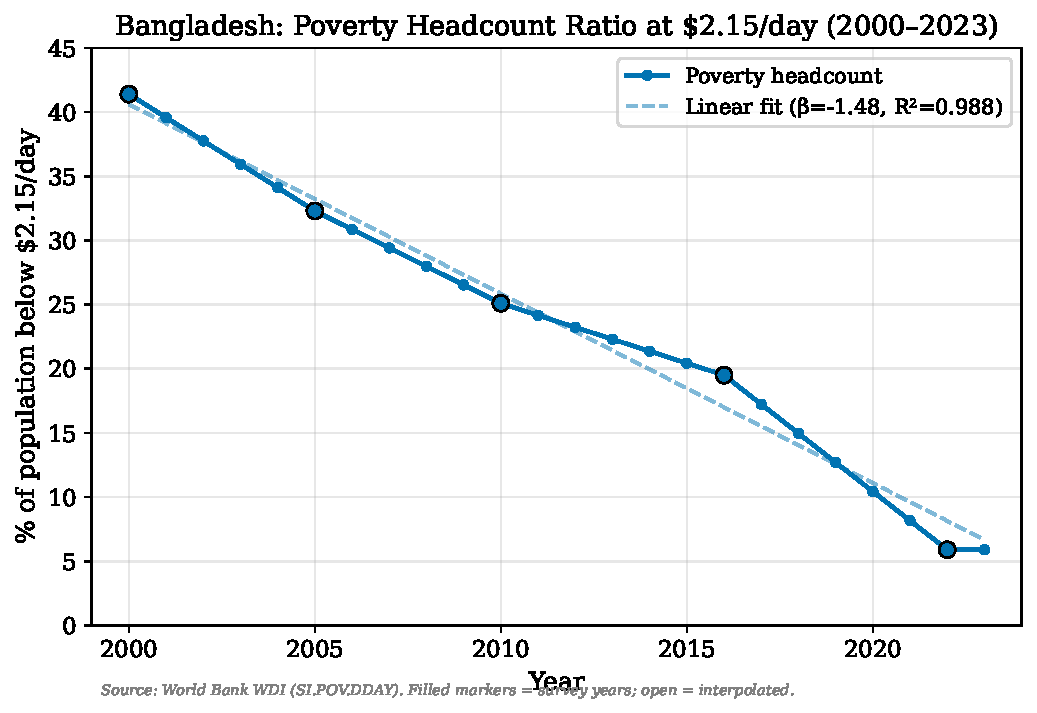
\includegraphics[width=0.85\textwidth]{../figures/fig1_poverty_trend.pdf}
\caption{Poverty headcount ratio at \$3.00/day, Bangladesh (2000--2023).}
\label{fig:poverty}
\end{figure}

\begin{figure}[H]
\centering
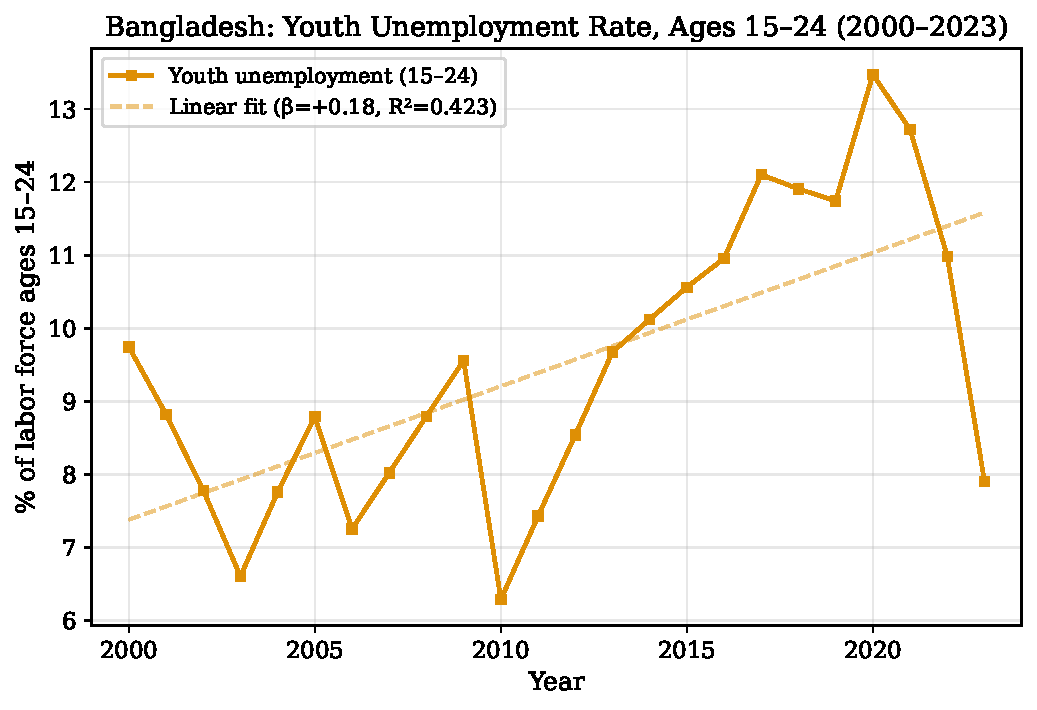
\includegraphics[width=0.85\textwidth]{../figures/fig2_unemployment_trend.pdf}
\caption{Youth unemployment rate (15--24), Bangladesh (2000--2023).}
\label{fig:unemployment}
\end{figure}

\begin{figure}[H]
\centering
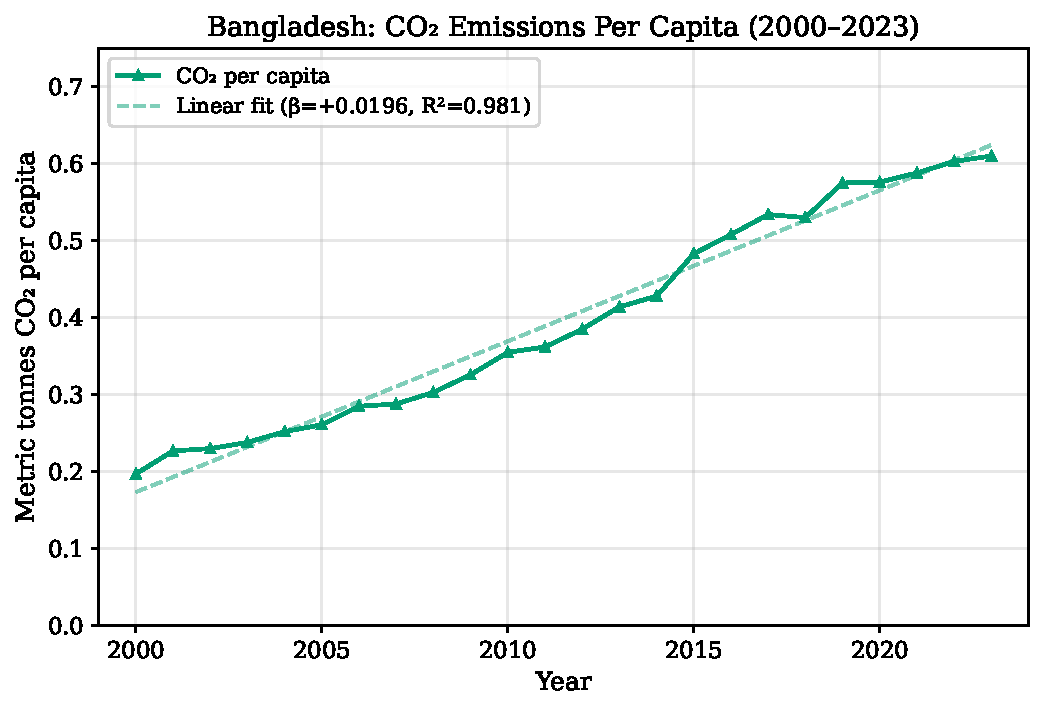
\includegraphics[width=0.85\textwidth]{../figures/fig3_co2_trend.pdf}
\caption{CO\textsubscript{2} emissions per capita, Bangladesh (2000--2023).}
\label{fig:co2}
\end{figure}

\subsection{3ZPI Composite Index}

\begin{table}[H]
\centering
\caption{3ZPI Trajectory (Selected Years)}
\label{tab:3zpi}
\begin{tabular}{rrrrr}
\toprule
Year & Poverty (norm) & Youth Unemp. (norm) & CO\textsubscript{2} (norm) & \textbf{3ZPI} \\
\midrule
2000 & 0.000 & 0.519 & 1.000 & \textbf{0.506} \\
2003 & 0.154 & 0.956 & 0.901 & \textbf{0.670} \\
2010 & 0.459 & 1.000 & 0.617 & \textbf{0.692} \\
2016 & 0.617 & 0.350 & 0.247 & \textbf{0.405} \\
2020 & 0.872 & 0.000 & 0.082 & \textbf{0.318} \\
2023 & 1.000 & 0.775 & 0.000 & \textbf{0.592} \\
\bottomrule
\end{tabular}
\end{table}

The 3ZPI peaked at 0.692 in 2010, declined to 0.318 in 2020, and recovered to 0.592 by 2023. The net change over 24 years is only +0.085. Figure~\ref{fig:3zpi} shows the full trajectory.

\begin{figure}[H]
\centering
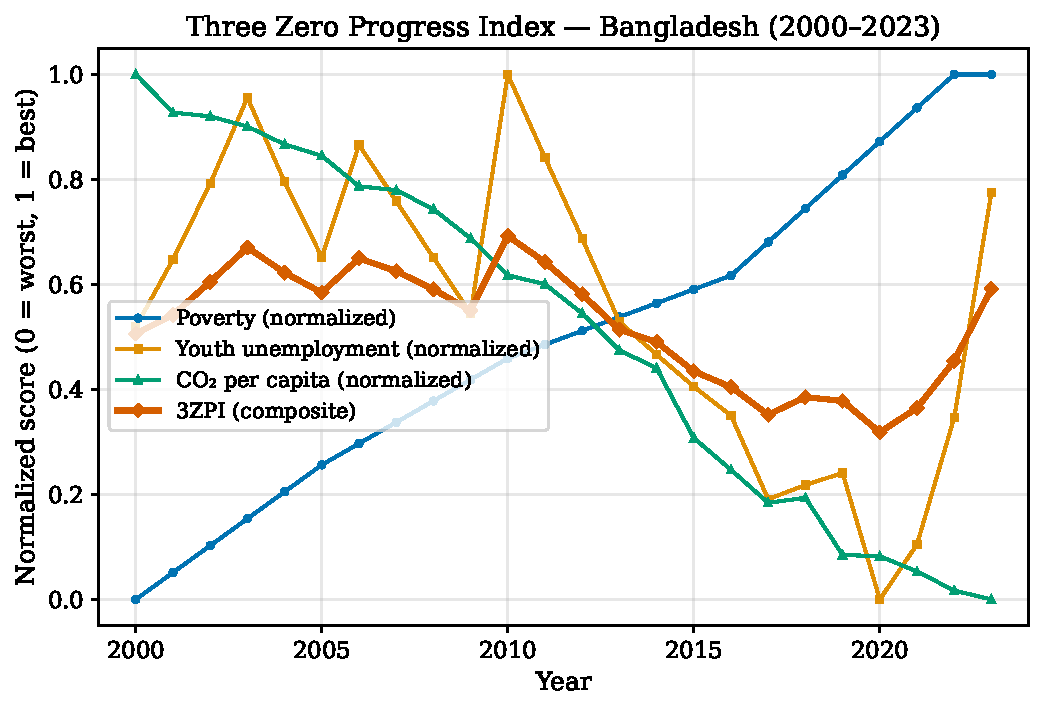
\includegraphics[width=0.85\textwidth]{../figures/fig4_three_zero_index.pdf}
\caption{Three Zero Progress Index and component indicators (2000--2023).}
\label{fig:3zpi}
\end{figure}

\subsection{Sensitivity Analysis}

\begin{table}[H]
\centering
\caption{3ZPI Under Alternative Weighting Schemes (Selected Years)}
\label{tab:sensitivity}
\begin{tabular}{rrrrr}
\toprule
Year & Equal & Poverty-heavy & Unemp-heavy & CO\textsubscript{2}-heavy \\
\midrule
2000 & 0.506 & 0.380 & 0.510 & 0.630 \\
2010 & 0.692 & 0.634 & 0.769 & 0.674 \\
2020 & 0.318 & 0.457 & 0.239 & 0.259 \\
2023 & 0.592 & 0.694 & 0.638 & 0.444 \\
\bottomrule
\end{tabular}
\end{table}

The qualitative conclusions are robust across all weighting schemes.

\subsection{Trend Analysis}

\begin{table}[H]
\centering
\caption{Linear Regression Results}
\label{tab:regression}
\begin{tabular}{lrrrr}
\toprule
Indicator & $\beta$ (annual) & $R^2$ & $p$-value & Projected year to zero \\
\midrule
Poverty (\%) & $-1.48$ & 0.988 & $<0.001$ & $\sim$2027 \\
Youth Unemp. (\%) & $+0.18$ & 0.423 & $<0.001$ & Never (trending up) \\
CO\textsubscript{2} pc (t) & $+0.020$ & 0.981 & $<0.001$ & Never (trending up) \\
\bottomrule
\end{tabular}
\end{table}

See Figure~\ref{fig:regression} for a comparison of regression slopes.

\begin{figure}[H]
\centering
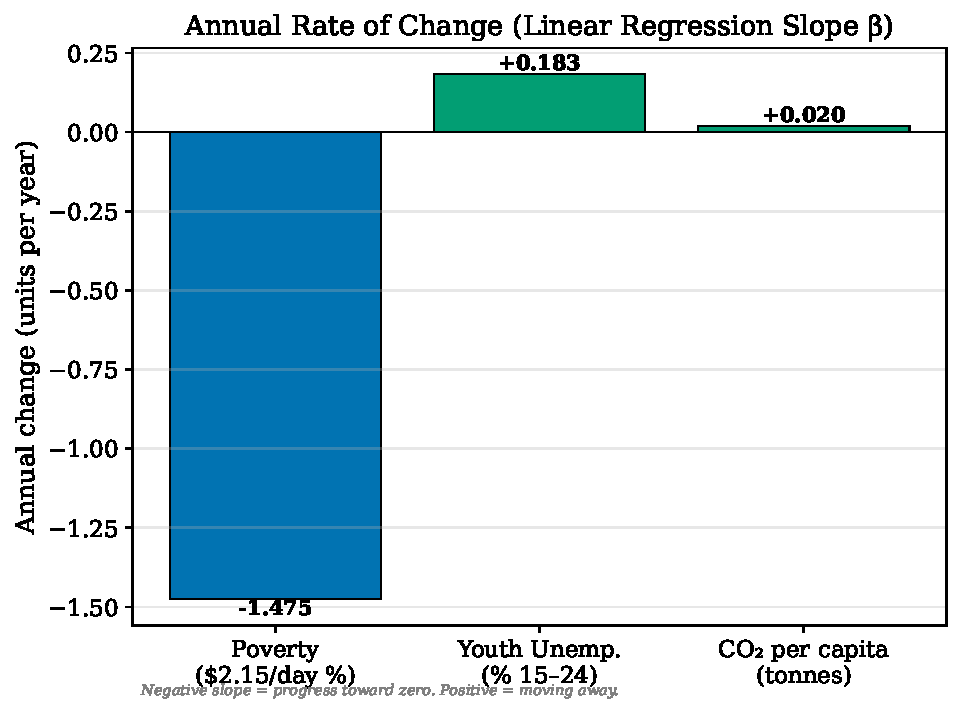
\includegraphics[width=0.75\textwidth]{../figures/fig6_regression_summary.pdf}
\caption{Annual rate of change (regression slope $\beta$) per indicator.}
\label{fig:regression}
\end{figure}

\subsection{Correlation Analysis}

\begin{table}[H]
\centering
\caption{Correlation Matrix (Normalized Scores)}
\label{tab:correlation}
\begin{tabular}{lrrr}
\toprule
 & Poverty & Youth Unemp. & CO\textsubscript{2} pc \\
\midrule
Poverty & 1.000 & $-0.620$ & $-0.978$ \\
Youth Unemp. & $-0.620$ & 1.000 & $+0.705$ \\
CO\textsubscript{2} pc & $-0.978$ & $+0.705$ & 1.000 \\
\bottomrule
\end{tabular}

\smallskip
\footnotesize All correlations exceed the 5\% significance threshold ($|r| > 0.404$, $df = 22$).
\end{table}

The near-perfect negative correlation ($r = -0.978$) between poverty and CO\textsubscript{2} is the central finding: the economic growth driving poverty reduction simultaneously worsens carbon performance. See Figure~\ref{fig:heatmap}.

\begin{figure}[H]
\centering
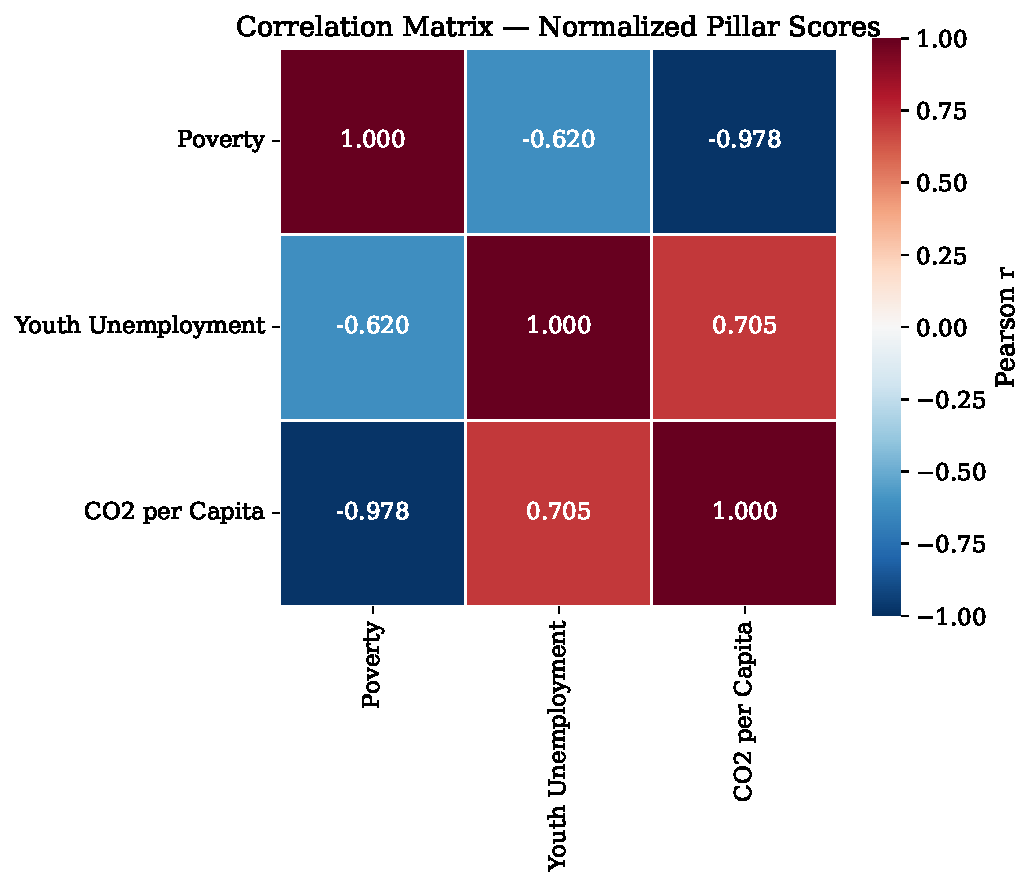
\includegraphics[width=0.65\textwidth]{../figures/fig5_correlation_heatmap.pdf}
\caption{Correlation heatmap of normalized pillar scores.}
\label{fig:heatmap}
\end{figure}

% ======================================================================
\section{Discussion}
% ======================================================================

\subsection{A Diverging Triangle}

The central finding is that Bangladesh's progress toward the three zeros is not just uneven --- it is actively divergent. The 3ZPI's modest net change of +0.085 over 24 years means that despite extraordinary poverty reduction, the overall 3 Zero progress has been limited because gains in one pillar were offset by losses in the other two.

The $r = -0.978$ correlation between poverty and CO\textsubscript{2} quantifies a structural tension: the way Bangladesh reduces poverty (fossil-fuel-powered industrialization) is fundamentally incompatible with the carbon target.

\subsection{Poverty: Extraordinary Progress}

The decline from 41.4\% to 5.9\% at the \$3.00/day line is one of the fastest sustained poverty reductions in the developing world. The linear projection suggests poverty at this threshold could approach zero by $\sim$2027, though the final percentage points will be the hardest.

\subsection{Youth Unemployment: Wrong Direction}

The positive regression slope ($+0.18$ pp/year) means youth unemployment is trending upward, not toward zero. The ``educated unemployment'' paradox and structural skills mismatch \citep{selim2021youth} suggest that economic growth alone is not solving the employment problem for young people.

\subsection{Carbon: The Structural Constraint}

CO\textsubscript{2} per capita tripled over the study period with a strong, consistent upward trend ($R^2 = 0.981$). Bangladesh's emissions are still low by global standards, but the trajectory is incompatible with any pathway to zero. Addressing this pillar requires changes beyond social business --- national energy policy and international climate finance are necessary \citep{stern2007}.

\subsection{Limitations}

Key limitations include: heavy interpolation of poverty data (5 survey points over 24 years); modeled rather than surveyed unemployment data; CO\textsubscript{2} source transition between World Bank and GCP; single-indicator-per-pillar design; and linear regression on 24 points providing descriptive rather than predictive power.

% ======================================================================
\section{Conclusion and Recommendations}
% ======================================================================

\subsection{Summary}

Bangladesh has made extraordinary progress on extreme poverty ($-$85\% at \$3.00/day) but youth unemployment is trending upward and CO\textsubscript{2} per capita has tripled. The composite 3ZPI moved only +0.085 over 24 years. A near-perfect negative correlation ($r = -0.978$) between poverty and carbon progress reveals that the current development model, while effective at reducing poverty, is structurally antagonistic to the carbon target.

\subsection{Recommendations}

For policymakers: (1) track the three goals together using a composite index; (2) treat youth unemployment as a structural problem requiring skills reform; (3) accelerate renewable energy and reconsider fossil fuel expansion.

For the 3 Zero Movement: (4) invest in green employment at the intersection of the unemployment and carbon pillars; (5) publish regular quantitative progress reports.

For future research: (6) expand to multiple indicators per pillar; (7) apply nonlinear models; (8) conduct subnational and multi-country analysis.

\subsection{Concluding Remarks}

The 3 Zero Progress Index is a simple tool --- min-max normalization, weighted averages, and linear regression. But applied to verified data and a well-defined question, it reveals that Bangladesh's development is deeply imbalanced. If the 3 Zero vision is to be realized, something has to change in how growth happens, not just how fast.

% ======================================================================
\bibliographystyle{plainnat}
\bibliography{references}

\end{document}
